\chapter{Resultados e Discussões}
\label{cap:resultados}
Este capítulo apresenta os resultados obtidos com a execução dos testes de carga descritas.

\section{Resultados}
Esta seção apresenta uma análise gráfica dos resultados obtidos com a execução dos testes de carga. Inicia-se pela abordagem \acrshort{ssr} (implementação \acrshort{mpa} em Next.js), considerando consumo de recursos no servidor (CPU e memória) e métricas de experiência do usuário (Web Vitals).

\subsection{Resultados para SSR}
\label{subsec:resultados-ssr}

A \autoref{fig:ssr-cpu} indica uso de CPU baixo e estável ao longo do teste, variando aproximadamente entre 8\% e 13\%, sem picos relevantes; a queda ao final corresponde ao encerramento do experimento.

\begin{figure}[H]
  \centering
  \caption{Média de uso de CPU por tempo (\acrshort{ssr})}
  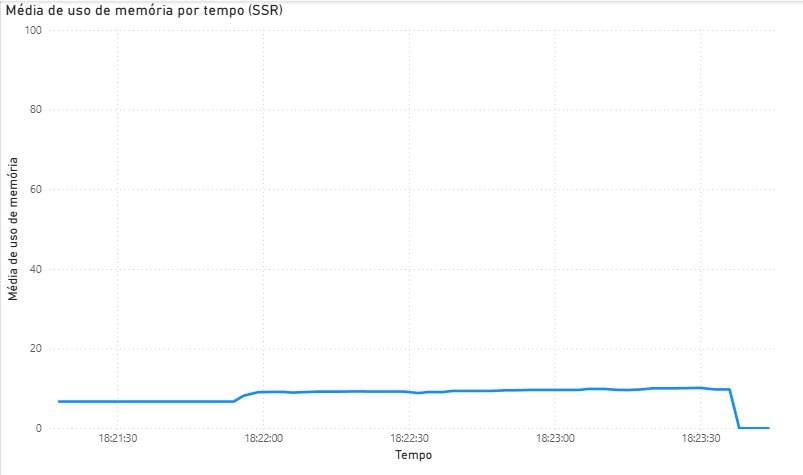
\includegraphics[width=0.9\textwidth]{media/uso_cpu_ssr.jpeg}
  \legend{Fonte: os autores.}
  \label{fig:ssr-cpu}
\end{figure}

A \autoref{fig:ssr-mem} mostra a média de uso de memória ao longo do teste. Nota-se um patamar estável (variação estreita) compatível com a execução do servidor Next.js, seguido de queda ao término do experimento.

\begin{figure}[H]
  \centering
  \caption{Média de uso de memória por tempo (\acrshort{ssr})}
  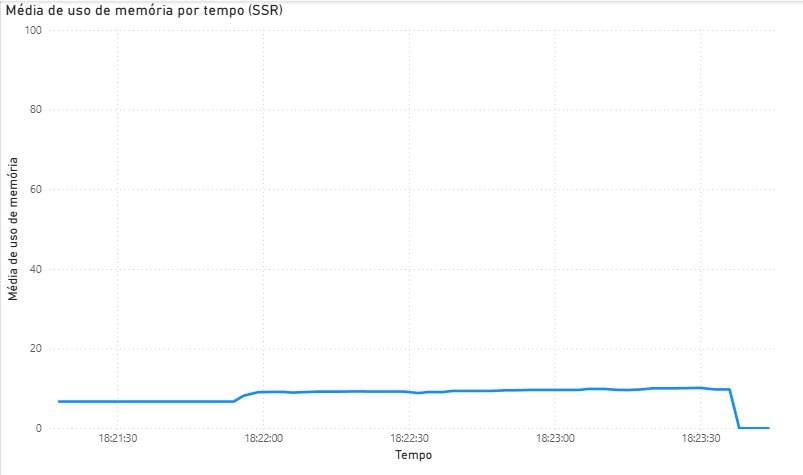
\includegraphics[width=0.9\textwidth]{media/uso_memoria_ssr.jpeg}
  \legend{Fonte: os autores.}
  \label{fig:ssr-mem}
\end{figure}


A \autoref{fig:ssr-webvitals} resume a classificação das \textit{Web Vitals} coletadas no cliente para a versão \acrshort{ssr}. Há predominância de resultados \textit{good}; identificam-se pequenas parcelas \textit{needs-improvement} em \acrshort{inp} e \acrshort{lcp}, e fração \textit{poor} em \acrshort{fcp}.

\begin{figure}[H]
  \centering
  \caption{Classificação das métricas de desempenho (\acrshort{ssr}) com Web Vitals}
  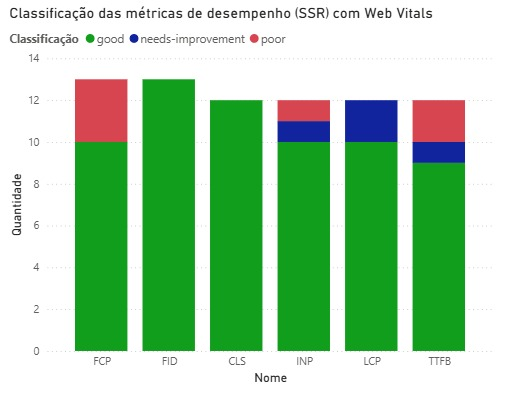
\includegraphics[width=0.9\textwidth]{media/metricas_ssr_web_vitals.jpeg}
  \legend{Fonte: os autores.}
  \label{fig:ssr-webvitals}
\end{figure}


\subsection{Resultados para CSR}
\label{subsec:resultados-csr}

A \autoref{fig:csr-cpu} apresenta a média de uso de CPU ao longo do teste da versão \acrshort{csr}. O consumo manteve-se \textit{muito baixo e estável}, com pequenas oscilações e picos inferiores a 5\%, sem indícios de saturação do host.

\begin{figure}[H]
  \centering
  \caption{Média de uso de CPU por tempo (\acrshort{csr})}
  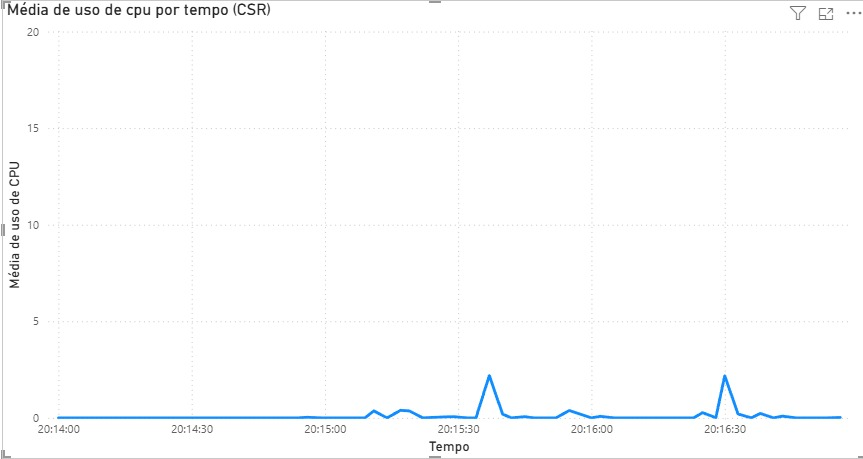
\includegraphics[width=0.9\textwidth]{media/uso_cpu_csr.jpeg}
  \legend{Fonte: os autores.}
  \label{fig:csr-cpu}
\end{figure}

A \autoref{fig:csr-mem} mostra a média de uso de memória durante o experimento. Observa-se um patamar \textit{muito baixo}, praticamente constante e inferior a 5\%, coerente com a entrega de conteúdo estático e execução de lógica no cliente.

\begin{figure}[H]
  \centering
  \caption{Média de uso de memória por tempo (\acrshort{csr})}
  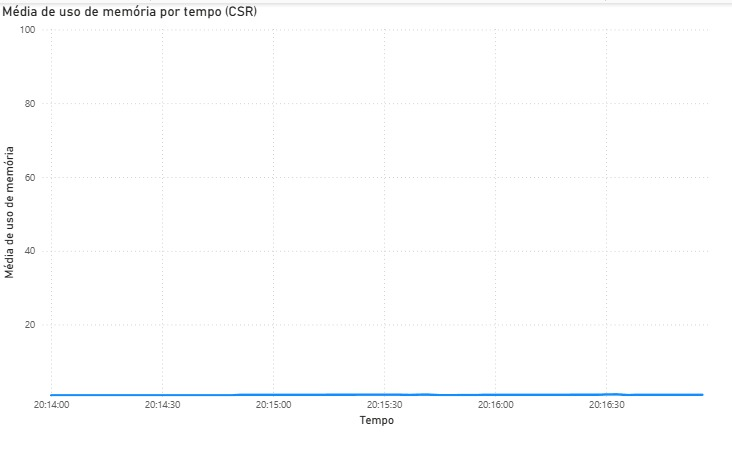
\includegraphics[width=0.9\textwidth]{media/uso_memoria_csr.jpeg}
  \legend{Fonte: os autores.}
  \label{fig:csr-mem}
\end{figure}

A \autoref{fig:csr-webvitals} resume a classificação das \textit{Web Vitals} para a versão \acrshort{csr}. As métricas \acrshort{ttfb}, \acrshort{fcp}, \acrshort{lcp} e \acrshort{inp} aparecem majoritariamente como \textit{good}. Em contraste, a \acrshort{cls} concentra ocorrências \textit{poor}, indicando \textit{layout shifts} durante o carregamento (por exemplo, imagens sem dimensões reservadas, fontes web sem \textit{preload} ou componentes que mudam de tamanho após hidratação).

\begin{figure}[H]
  \centering
  \caption{Classificação das métricas de desempenho (\acrshort{csr}) com Web Vitals}
  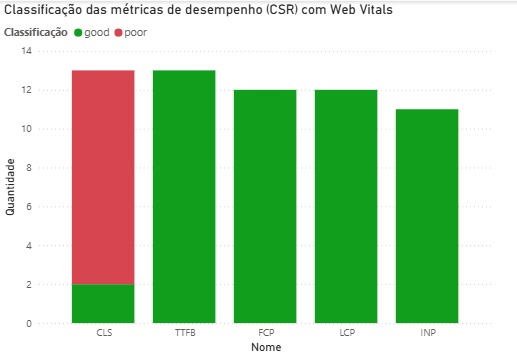
\includegraphics[width=0.9\textwidth]{media/metricas_csr_web_vitals.jpeg}
  \legend{Fonte: os autores.}
  \label{fig:csr-webvitals}
\end{figure}

\subsection{Comparação entre SSR e CSR}
\label{subsec:comparacao-ssr-csr}

A Tabela~\ref{tab:comparativo-ssr-csr} sintetiza os achados principais observados nas Figuras \autoref{fig:ssr-cpu}--\autoref{fig:ssr-webvitals} (SSR) e \autoref{fig:csr-cpu}--\autoref{fig:csr-webvitals} (CSR).

\begin{table}[H]
\centering
\caption{Síntese comparativa dos resultados (SSR $\times$ CSR) neste estudo}
\label{tab:comparativo-ssr-csr}
\begin{tabular}{|p{4.0cm}|p{5.2cm}|p{5.2cm}|}
\hline
\textbf{Aspecto} & \textbf{SSR (MPA/Next.js)} & \textbf{CSR (SPA/React)} \\
\hline
\textbf{CPU no servidor} & Baixa e estável, \textit{$\sim$8--13\%} em média, sem picos relevantes. & Muito baixa, oscilações discretas com picos $<5\%$. \\
\hline
\textbf{Memória no servidor} & Patamar estável com variação estreita (\textit{cerca de} 8--15\%), queda ao término do teste. & Muito baixa e praticamente constante ($<5\%$). \\
\hline
\textbf{Web Vitals (cliente)} & Predominância de \textit{good}; pequenos trechos \textit{needs-improvement} em \acrshort{lcp}/\acrshort{inp} e fração \textit{poor} em \acrshort{fcp}. & \acrshort{ttfb}, \acrshort{fcp}, \acrshort{lcp} e \acrshort{inp} majoritariamente \textit{good}; \textbf{\acrshort{cls} com ocorrências \textit{poor}}. \\
\hline
\textbf{Interpretação} & Parte do trabalho de renderização é feita no servidor, o que eleva discretamente CPU/memória, mas favorece \textit{TTFB}/exibição inicial. \acrshort{lcp}/\acrshort{inp} podem sofrer com \textit{hydration} e imagens. & Lógica e montagem no cliente aliviam o servidor; porém, maior risco de \acrshort{cls} por mudanças de layout durante carregamento/hidratação e falta de reserva de espaço. \\
\hline
\end{tabular}
\end{table}

\subsection{Discussão}
(i) \textbf{Recursos do servidor.} O \acrshort{ssr} apresentou consumo levemente maior de CPU e memória (ainda baixo) em relação ao \acrshort{csr}, o que é esperado pelo processamento por requisição no servidor.
(ii) \textbf{Experiência do usuário.} Em \acrshort{ssr}, os resultados indicam boa experiência geral, com atenção a \acrshort{lcp}/\acrshort{inp}, possivelmente impactados por imagens e trabalho de \textit{hydration}. Em \acrshort{csr}, as Web Vitals também ficaram majoritariamente em \textit{good}, com exceção da \textbf{\acrshort{cls}}, sinalizando \textit{layout shifts} durante o carregamento.

\subsection{Implicações práticas.}
\begin{itemize}
  \item \textbf{Quando priorizar SSR:} páginas públicas e sensíveis a \acrshort{seo}, conteúdo editorial e e-commerce, quando a exibição rápida de HTML e o \acrshort{ttfb} consistente são críticos.
  \item \textbf{Quando priorizar CSR:} aplicações altamente interativas (dashboards, apps internos) em que a carga sobre o servidor deva ser mínima e a navegação contínua no cliente seja preferível.
\end{itemize}

\subsection{Ajustes recomendados.}
\textbf{Para SSR (melhorar \acrshort{lcp}/\acrshort{inp}):} otimização e dimensionamento de imagens (lazy/\texttt{priority} para \textit{hero}), \textit{streaming} e/ou \textit{partial hydration}, redução de JS não crítico, uso de \textit{server components} e \texttt{preload}/\texttt{dns-prefetch} para recursos críticos.  
\textbf{Para CSR (mitigar \acrshort{cls}):} reservar dimensões de mídia (\texttt{width}/\texttt{height} ou \texttt{aspect-ratio}); evitar inserções acima da dobra após a montagem; \texttt{font-display: swap} com \textit{preload} de fontes; placeholders com tamanho final; adiar banners/consentimentos para abaixo da dobra.

\subsection{Síntese.}
No cenário testado, ambos os modelos atenderam com folga aos recursos do host. O \acrshort{ssr} entrega conteúdo inicial rapidamente, mas requer cuidado com \acrshort{lcp}/\acrshort{inp} ligados à hidratação; o \acrshort{csr} minimiza o custo no servidor, porém demanda disciplina para eliminar \acrshort{cls}. A escolha deve considerar \acrshort{seo}, tipo de interação e perfil de tráfego, aplicando as otimizações citadas para mitigar as fraquezas de cada abordagem.
